\thispagestyle{empty}
\definecolor{Gray2}{rgb}{ .851,  .851,  .851}
\chapter{Vuelo Horizontal}

\spacing{1.5}

Las condiciones para el vuelo rectilíneo son sencillas, la velocidad vertical ha de ser nula mientras que la horizontal no. Con estas condiciones y a nivel del mar se pueden obtener las gráficas \ref{PMVH}, \ref{ControlVH}, \ref{EulerVH} y \ref{PVH}, que ofrecen una primera aproximación del rendimiento de la aeronave. De ellas se puede obtener que el valor de potencia total mínimo es de 27,307 kW, y se da para una velocidad de vuelo de 28.73 m/s. Este valor resulta de especial interés ya que nos ofrece el vuelo de máxima autonomía,muy interesante en misiones de vigilancia.

\begin{figure}
	\centering
	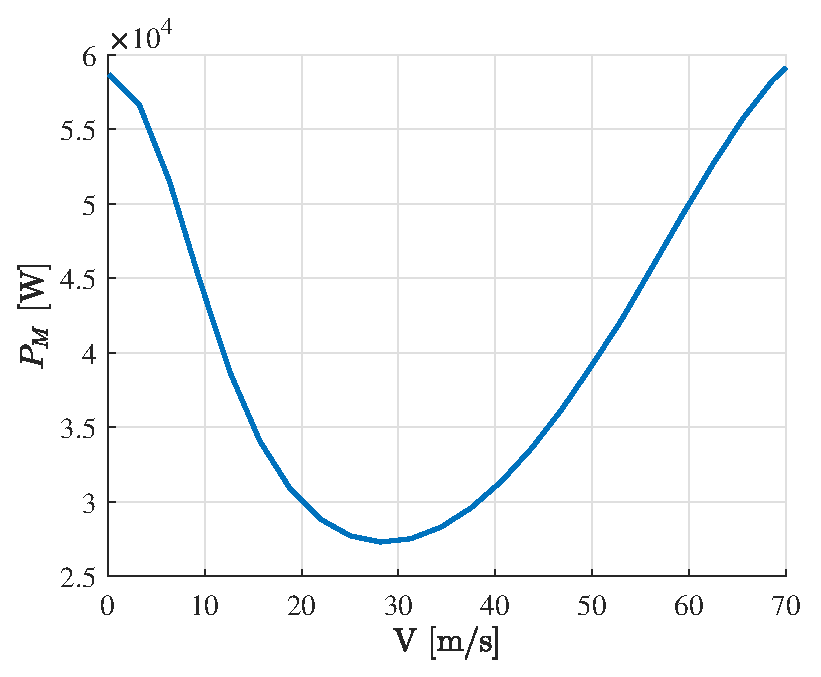
\includegraphics[width=90mm]{graficos/PMVH}
	\caption{Consumo de Potencia de la aeronave en función de la velocidad de vuelo a nivel del mar para vuelo horizontal y limitación por potencia máxima continua disponible.}
	\label{PMVH}
\end{figure}
\begin{figure}
	\centering
	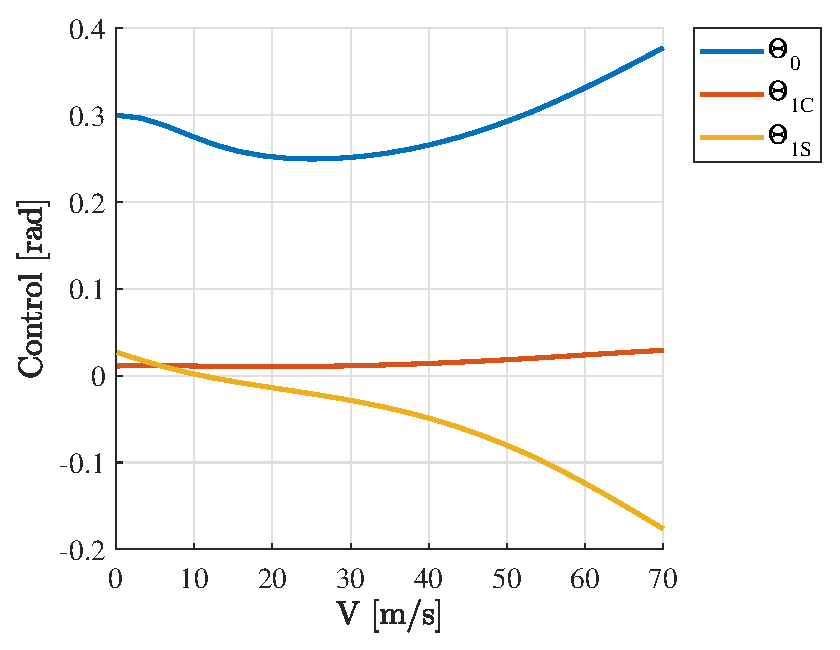
\includegraphics[width=90mm]{graficos/ControlVH}
	\caption{Ángulos de control de la aeronave en función de la velocidad de vuelo a nivel del mar para vuelo horizontal}
	\label{ControlVH}
\end{figure}
\begin{figure}
	\centering
	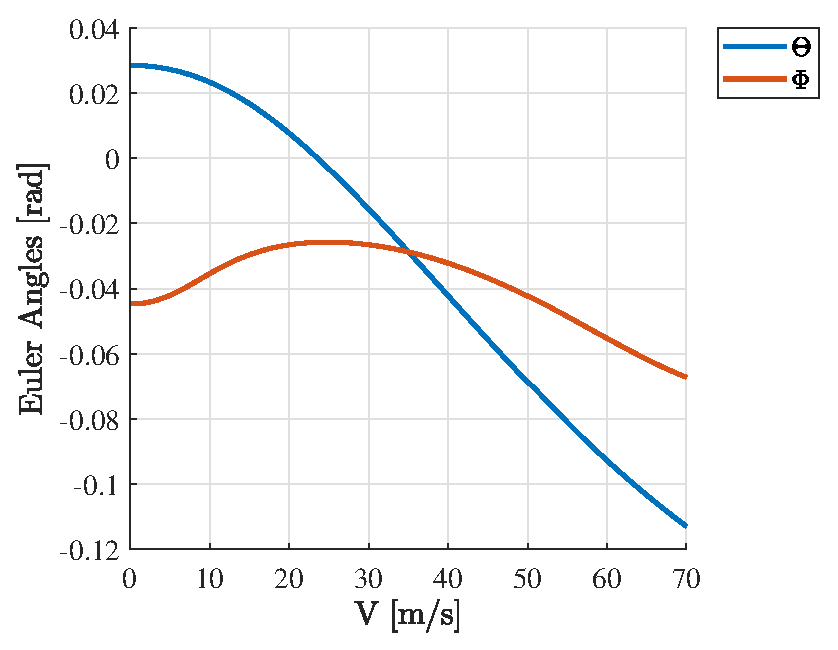
\includegraphics[width=90mm]{graficos/EulerVH}
	\caption{Ángulos de Euler de la aeronave en función de la velocidad de vuelo a nivel del mar para vuelo horizontal}
	\label{EulerVH}
\end{figure}
\begin{figure}
	\centering
	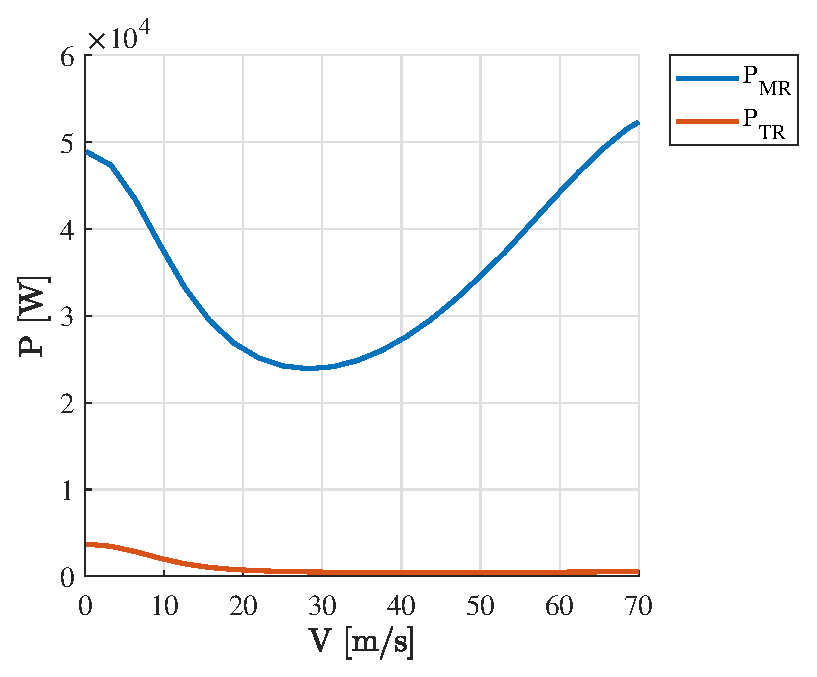
\includegraphics[width=90mm]{graficos/PVH}
	\caption{Consumo de Potencia de los rotores principal y antipar en función de la velocidad de vuelo a nivel del mar para vuelo horizontal}
	\label{PVH}
\end{figure}

\section{Autonomía de Vuelo}

Con estos datos se puede hacer una estimación de la autonomía del vehículo. Para ello es necesario obtener características del motor, el cual no se ha decidido, por lo que, para tener unos valores orientativos, se ha optado por emplear los datos del motor que monta el Cicaré 7B, un helicóptero de peso similar al vehículo a diseñar. El motor en cuestión es el ROTAX 912 ULS, un motor de 4 tiempos y 4 cilindros, con un consumo especifico de 285 g/kW$\cdot$ h a una potencia máxima continua de 58 kW a 5500 rpm \citep{ROTAX}.
Para poder obtener el consumo específico del motor en las condiciones de vuelo de máxima autonomía,se emplea el modelo recogido en \citet{Cuerva}, que modeliza el consumo en función de la potencia necesaria para el vuelo.
\begin{equation}
	c_e(P)=\frac{c_{e,P_{max}}}{1+\frac{K_m}{c_{e,P_{max}}}(1-\frac{P_{max}}{P(t)})}
	\label{consumo}
\end{equation}
Donde $c_e$ es el consumo específico al régimen de vuelo considerado, $c_{e,P_{max}}$ el consumo específico del motor en régimen de funcionamiento de máxima potencia, $P_{max}$ la potencia máxima continua capaz de ofrecer el motor y $P$ la potencia necesaria para el vuelo considerado.
$K_m$ es un parámetro que mide la eficiencia del motor, que en motores muy eficientes es del orden de 8.33$\cdot$10$^-9$ kg/W$\cdot$s (0.03 kg/kW$\cdot$h).
Además se suponen unas cargas de combustible del 9\% del MTOW del vehículo. 

Lo siguiente es decidir un modelo de cálculo de la autonomía, ya que no se dispone de datos suficientes para hacer unos cálculos exactos,ni estos son necesarios en una fase de diseño preliminar. La hipótesis básica es considerar las masa del vehículo constante durante el vuelo, cosa que no es así por el consumo del propio combustible, pero simplificará los cálculos en gran medida.
Para los cálculos se empleará el método del equilibrado del helicóptero, que permite incluir gran cantidad de información en los cálculos y por tanto aumentar la fiabilidad de estos. Como se desarrollará a continuación, la complejidad de este método reside en el propio equilibrado del helicóptero, que permitirá obtener el valor de potencia requerido para el vuelo, a partir del cual el cálculo de la autonomía resulta trivial.

En \citet{Filippone} se expone un método para calcular la autonomía de forma sencilla empleando para ello la potencia (calculada mediante el equilibrado) del vuelo y el consumo específico (calculado mediante la ecuación \ref{autonomia}).
Se define la autonomía específica $E_s$
\begin{equation}
	E_s=\frac{\partial t}{\partial m}=\frac{1}{\dot{m_f}}=\frac{1}{P\cdot c_{e}(P)}
	\label{autespecifica}
\end{equation}
y con la hipótesis de masa constante solo es necesario resolver el equilibrado para una velocidad ya que
\begin{equation}
	\frac{\partial P}{\partial t}=0\rightarrow P=cte
\end{equation}
que al introducir en la ecuación \ref{consumo} se obtiene que
\begin{equation}
	P=cte\rightarrow c_e=cte
\end{equation}
y por tanto
\begin{equation}
E_s=\frac{1}{P\cdot c_{e}}=cte
\label{autespecificacte}
\end{equation}
Una vez obtenido el valor de la autonomía especifica, el calculo de la autonomía resulta sencillo
\begin{equation}
	t_{e}=E_s\cdot \Delta m=E_s\cdot MFM=\frac{MFM}{c_e\cdot P}
	\label{autonomia}
\end{equation}

Donde $t_e$ es la autonomía, $MFM$ es la masa máxima de combustible, $C_{e}$ es el consumo específico y $P_e$ la potencia en el régimen de de vuelo.
La tabla \ref{auttabla} recoge los datos necesarios para el cálculo de la autonomía máxima y el valor de esta.

\begin{table}[htbp]
	\centering
	\begin{tabular}{|>{\columncolor{Gray}}c|c|}
		\hline
		\cellcolor{Gray2}Variable & \cellcolor{Gray2}Valor \\ \hline \hline
		\cellcolor{Gray}Potencia para máxima autonomía ($P_{min,t_{e,max}}$)  & 27.307 kW \\ \hline
		\cellcolor{Gray}Velocidad en régimen de máxima autonomía ($V$) & 28.73 m/s \\ \hline
		\cellcolor{Gray}Consumo específico en régimen de máxima autonomía ($c_{e,t_{e,max}}$) & 8.98$\cdot$10$^-08$ kg/W$\cdot$s \\ \hline
		\cellcolor{Gray}Máxima autonomía ($t_{e,max}$) & 4.588 h \\ \hline
	\end{tabular}%
	\caption{Valores de inercia del helicóptero semilla.}
	\label{auttabla}
\end{table}%

A modo de comprobación, se han calculado las autonomías correspondientes a distintas velocidades de vuelo en la gráfica \ref{teVH}. Se puede observar que su forma resulta muy similar a la de la gráfica \ref{PMVH} pero invirtiéndola según el eje x. Esto se debe a que la autonomía no depende de otro parámetro de vuelo que no sea la potencia consumida, por lo que la evolución de la potencia necesaria será inversa a la evolución de la autonomía de vuelo, siendo el mínimo de potencia necesaria el máximo de autonomía.

\begin{figure}
	\centering
	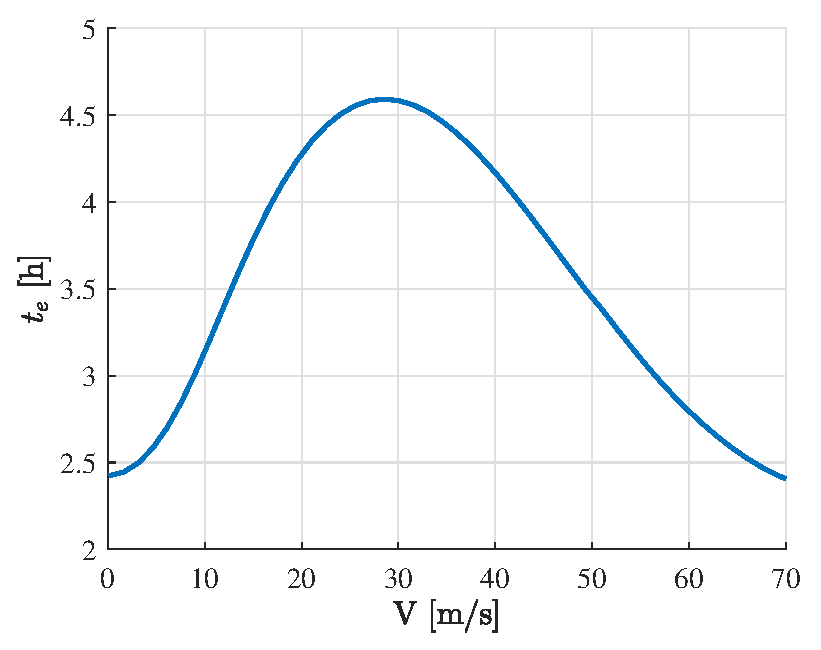
\includegraphics[width=90mm]{graficos/teVH}
	\caption{Autonomía de la aeronave en función de la velocidad de vuelo a nivel del mar para vuelo horizontal.}
	\label{teVH}
\end{figure}
%Los datos del motor son
%Pot. Max. Coontinua 58 Kw
%consumo l/h 22,6 (100%) y 16,2 (75%)
%consumo especifico al 100% 285g/kWh
%Con el la potencia de máxima autonomía a 31,5kW, una regla de 3 nos dice que el consumo es un 51.9069026% del de maxima potencia,regla de 3, no 100% seguro.

\section{Fuerzas y Momentos Sobre los Elementos de la Estructura}

En futuras fases de diseño será necesario definir el diseño estructural y los materiales con los que se construirá la aeronave, por lo que puede ser interesante realizar un análisis de las fuerzas que deberán soportar algunos elementos para tener una idea aproximada de las cargas que pueden aparecer en servicio.

De entre estas cargas, las que aparecen en los elementos de la cola son muy importantes, ya que los momentos flectores inducidos por estas cargas en la propia cola pueden ser grandes debido a la longitud de esta, y habrá que diseñarla de tal manera que las posibles deformaciones que aparezcan en funcionamiento no interfieran en el mismo.

Las figuras \ref{FAP} y \ref{FE} representan los valores de las fuerzas que aparecen en el rotor antipar y estabilizadores vertical y horizontal para cada velocidad de vuelo considerada. Solo se representas las cargas que tienen algún valor de interés, por ejemplo, las cargas en el eje y que se den en el estabilizador horizontal serán despreciables y no serán relevantes a la hora de calcular las cargas sobre la cola.

\begin{figure}
	\centering
	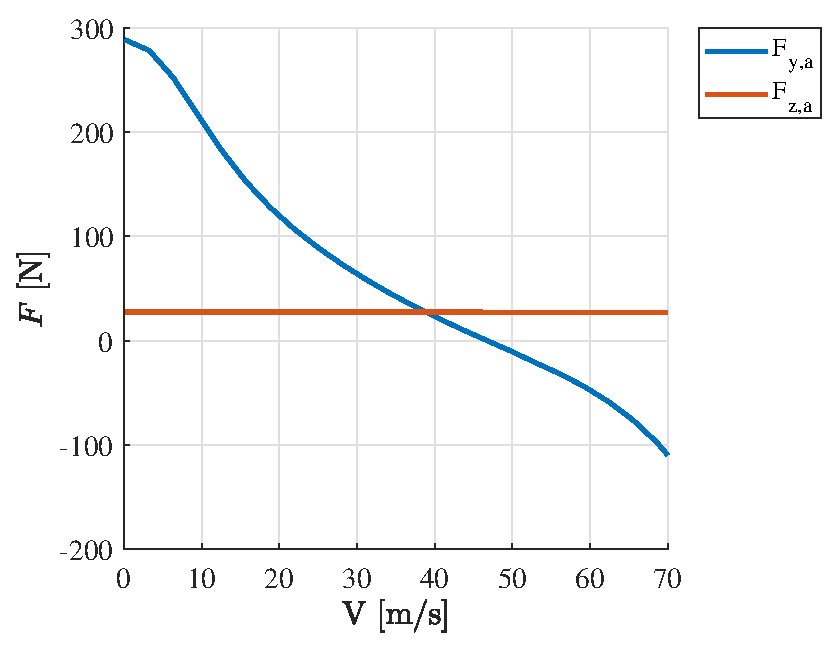
\includegraphics[width=90mm]{graficos/FAP}
	\caption{Fuerzas sobre el rotor antipar a distintas velocidades de vuelo a nivel del mar según los ejes y y z.}
	\label{FAP}
\end{figure}

\begin{figure}
	\centering
	\subfigure[Estabilizador vertical]{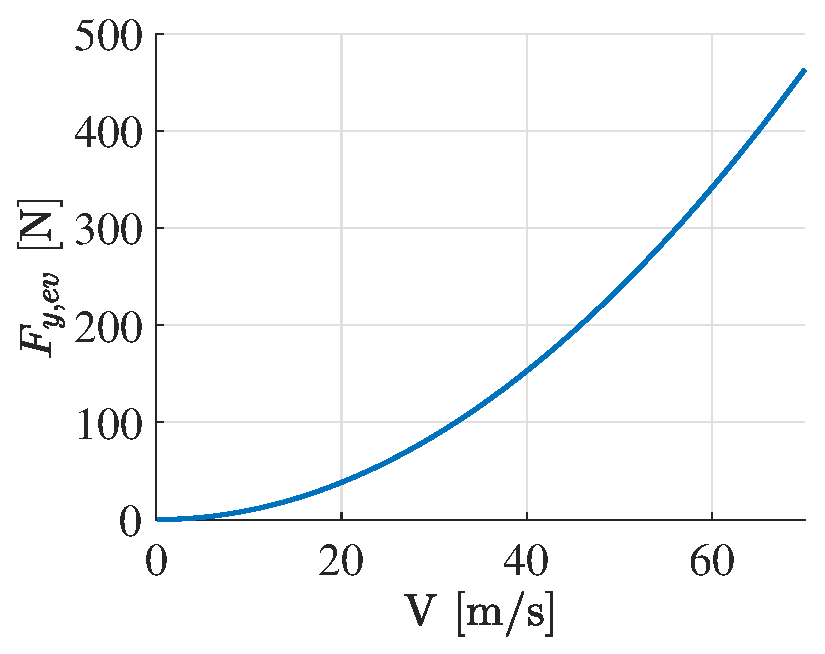
\includegraphics[width=60mm]{graficos/FEV}}
	\subfigure[Estabilizador horizontal]{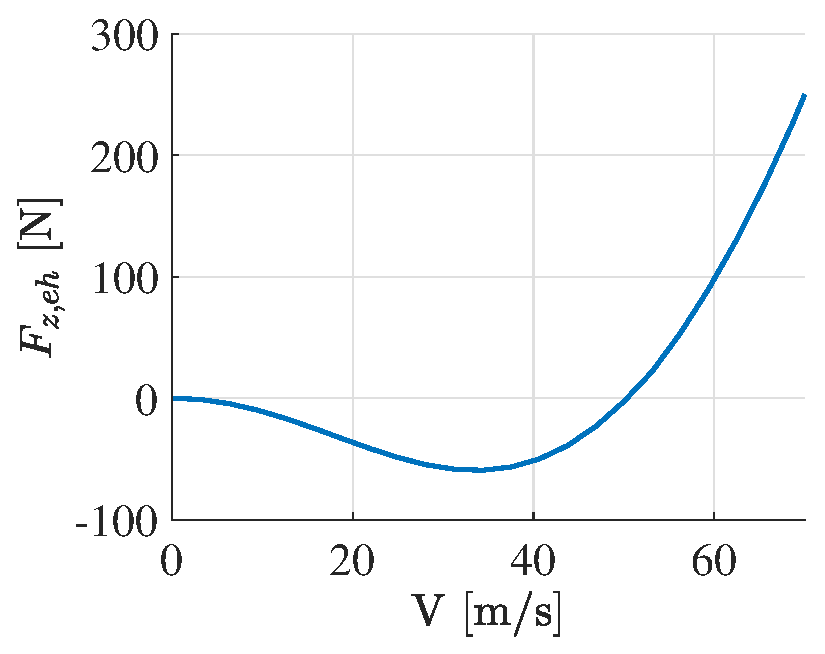
\includegraphics[width=60mm]{graficos/FEH}}
	\caption{Fuerzas sobre los estabilizadores (a) vertical y (b) horizontal a distintas velocidades de vuelo a nivel del mar. Las fuerzas que se representan son horizontales (eje y) para el estabilizador vertical y verticales (eje z) para el estabilizador vertical.}
	\label{FE}
\end{figure}


Se puede observar en la gráfica \ref{FAP} que las cargas sobre el rotor antipar cambian de signo, es decir, de sentido, a partir de ciertas velocidades. Esta evolución puede resultar extraña, pero el motivo se puede observar en la gráfica \ref{FAP}. Como ocurriría con un ala, el estabilizador vertical genera una carga en el eje y que aumenta con la velocidad de vuelo. Esta carga ayuda a reducir la potencia necesaria en el rotor antipar para bajas velocidades ya que ayuda a compensar el momento de giro que provoca el rotor principal. Sin embargo, estas cargas, para velocidades altas, superan a las necesarias para compensar dicho momento, y el antipar debe pasar a compensar la carga sobre el estabilizador vertical. Además, aunque su origen no es aerodinámico, el propio peso del rotor antipar supondrá una carga de valor constante que también se ha de tener en cuenta.

En lo que respecta al estabilizador horizontal, a bajas velocidades genera una carga ascendente que ayuda a la estabilidad longitudinal del sistema. A altas velocidades (mayores a 50 m/s) las cargas se vuelven descendentes. Esto puede deberse a un fallo del modelo, que en situaciones límite no sea capaz de obtener buenas aproximaciones, aunque en una situación real en avance, la estela del rotor principal puede incidir sobre el estabilizador horizontal y generar cargas descendentes.

Queda por tanto claro que a mayor velocidad de vuelo las cargas serán mayores, llegando hasta cargas de 300 N que la cola tendrá que soportar en vuelo a punto fijo (debidas al rotor antipar), pero mayores para vuelos a altas velocidades (400 N para vuelos a 60 m/s).


Estas simulaciones se han realizado suponiendo ángulos de ataque del fuselaje nulos, por lo que puede resultar interesante ver como evolucionan las cargas sobre los estabilizadores con el ángulo de ataque $\alpha_0$ y el ángulo de resbalamiento $\beta_f$. La gráfica \ref{FEa} representa la variación más significativa de las cargas en los estabilizadores, las cargas sobre el estabilizador horizontal. Se aprecia que su comportamiento es el de un perfil aerodinámico, incluso se aprecia un comportamiento prácticamente lineal con el ángulo de ataque. Todo esto implica que si se desean reducir las cargas en la cola, conviene volar a pequeños ángulos de ataque negativos, lo que, como se representa en la figura \ref{PMVHa}, conlleva un aumento de la potencia necesaria y por tanto del consumo a la par que una reducción de la autonomía de vuelo.

\begin{figure}
	\centering
	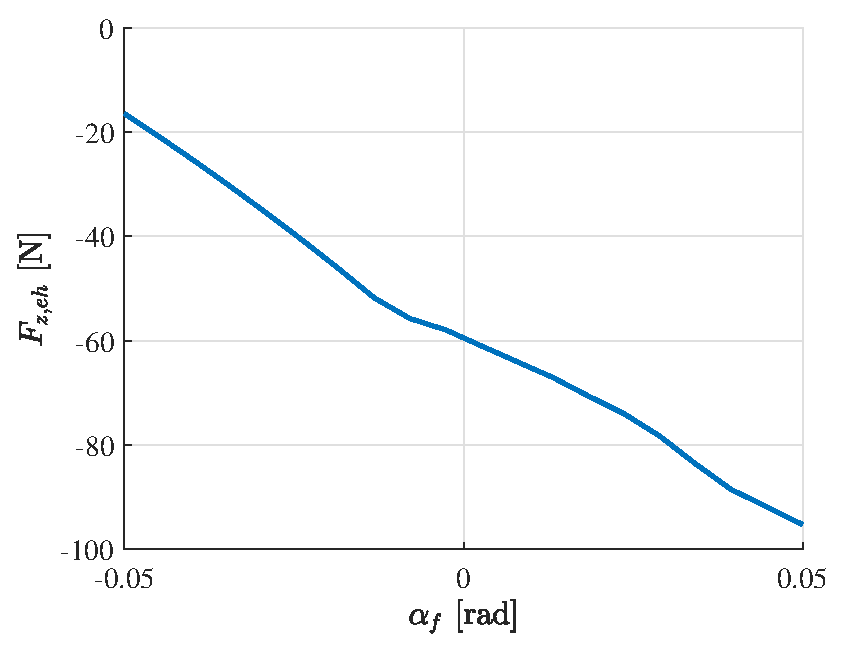
\includegraphics[width=90mm]{graficos/FEHa}
	\caption{Fuerzas sobre el estabilizador horizontal a distintos ángulos de ataque a nivel del mar para una velocidad de vuelo de 28 m/s.}
	\label{FEa}
\end{figure}

\begin{figure}
	\centering
	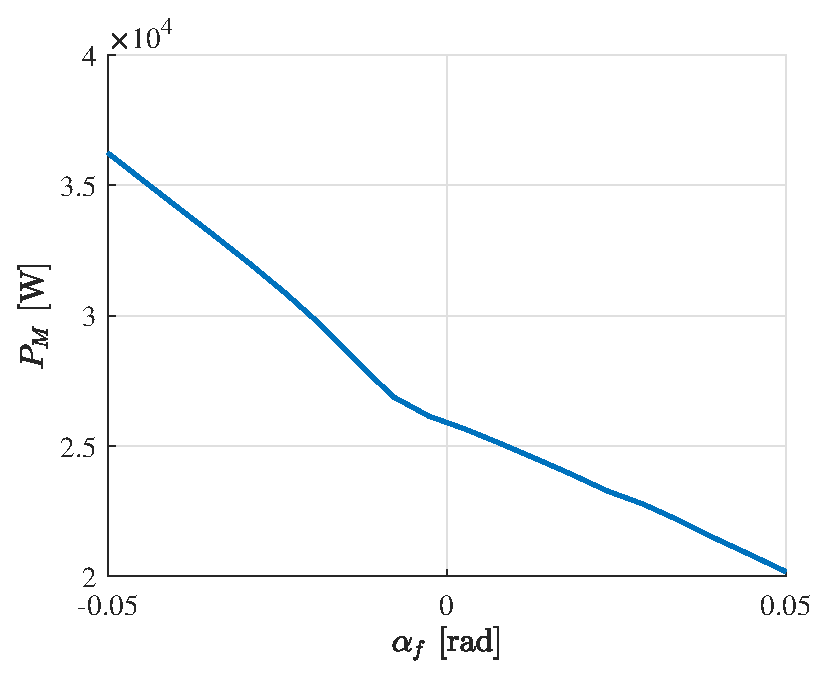
\includegraphics[width=90mm]{graficos/PMVHa}
	\caption{Potencia necesaria para un vuelo horizontal a distintos ángulos de ataque a nivel del mar para una velocidad de vuelo de 28 m/s.}
	\label{PMVHa}
\end{figure}

En estas circunstancias reducir el ángulo de ataque no resulta interesante, apenas variamos las cargas a costa de reducir la autonomía, pero si consideramos un vuelo con un ángulo de ataque $\alpha_f=0.025$ rad la autonomía se incrementa hasta las 5 horas y 20 minutos. Los resultados de estos cálculos se pueden encontrar en la tabla \ref{auttab2}.

\begin{table}[htbp]
	\centering
	\begin{tabular}{|>{\columncolor{Gray}}c|c|}
		\hline
		\cellcolor{Gray2}Variable & \cellcolor{Gray2}Valor \\ \hline \hline
		\cellcolor{Gray}Ángulo de ataque del fuselaje ($\alpha_f$)  & 0.025 rad \\ \hline
		\cellcolor{Gray}Velocidad de vuelo ($V$) & 28.73 m/s \\ \hline
		\cellcolor{Gray}Potencia necesaria ($PM$)  & 22.155 kW \\ \hline
		\cellcolor{Gray}Consumo específico ($c_{e}$) & 9.54$\cdot$10$^-08$ kg/W$\cdot$s \\ \hline
		\cellcolor{Gray}Autonomía ($t_{e,max}$) & 5.3231 h \\ \hline
	\end{tabular}%
	\caption{Valores de inercia del helicóptero semilla.}
	\label{auttab2}
\end{table}%

\begin{figure}
	\centering
	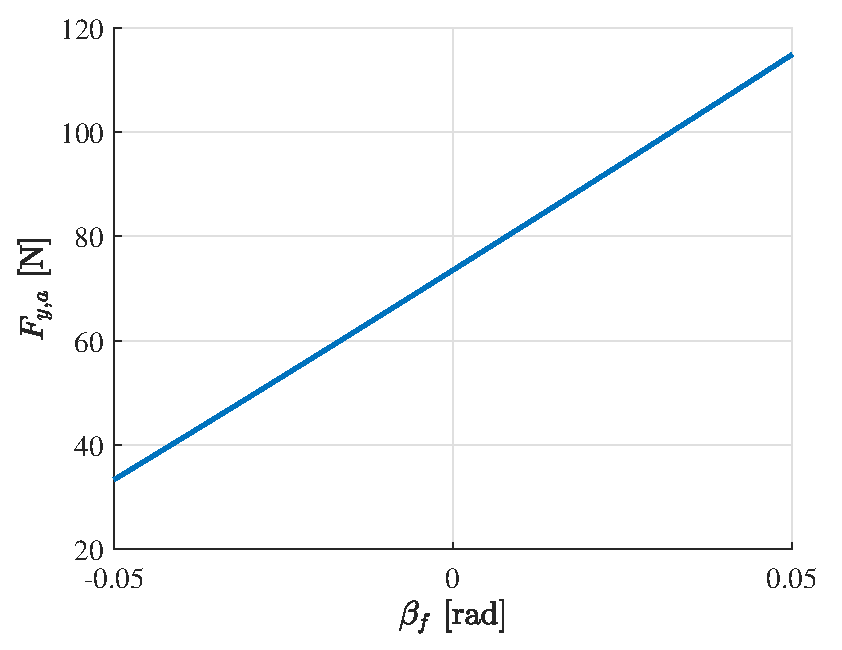
\includegraphics[width=90mm]{graficos/FAPb}
	\caption{Fuerzas sobre el rotor antipar a distintos ángulos de resbalamiento a nivel del mar para un vuelo horizontal a 28 m/s.}
	\label{FAPb}
\end{figure}

\begin{figure}
	\centering
	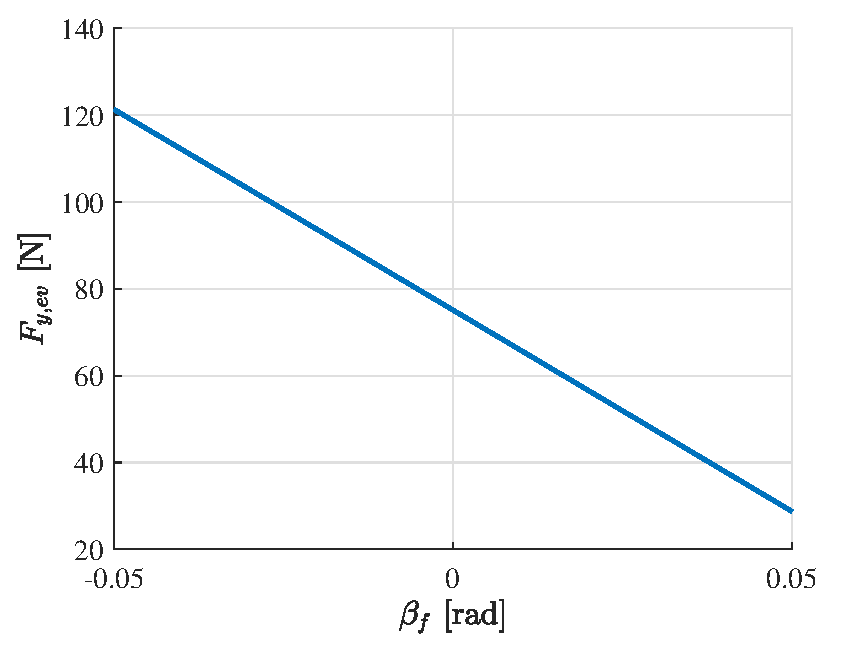
\includegraphics[width=90mm]{graficos/FEVb}
	\caption{Fuerzas sobre el estabilizador vertical a ángulos de resbalamiento a nivel del mar para un vuelo horizontal a 28 m/s.}
	\label{FEb}
\end{figure}



\singlespacing